\documentclass[a4paper, 12pt]{article}
\usepackage[T1]{fontenc}
\usepackage[utf8]{inputenc}
\usepackage[english]{babel}
\usepackage{graphicx}
\usepackage{minted}
\usepackage{graphicx}
\usepackage{subcaption}
\usepackage{setspace}
%\usepackage{listings}

\onehalfspacing

\begin{document}

\title{Very Large Scale Integration}
\author{G. Berselli, M. M. L. Pulici}
\date{August 29, 2021}
\maketitle
\begin{center}
	\fbox{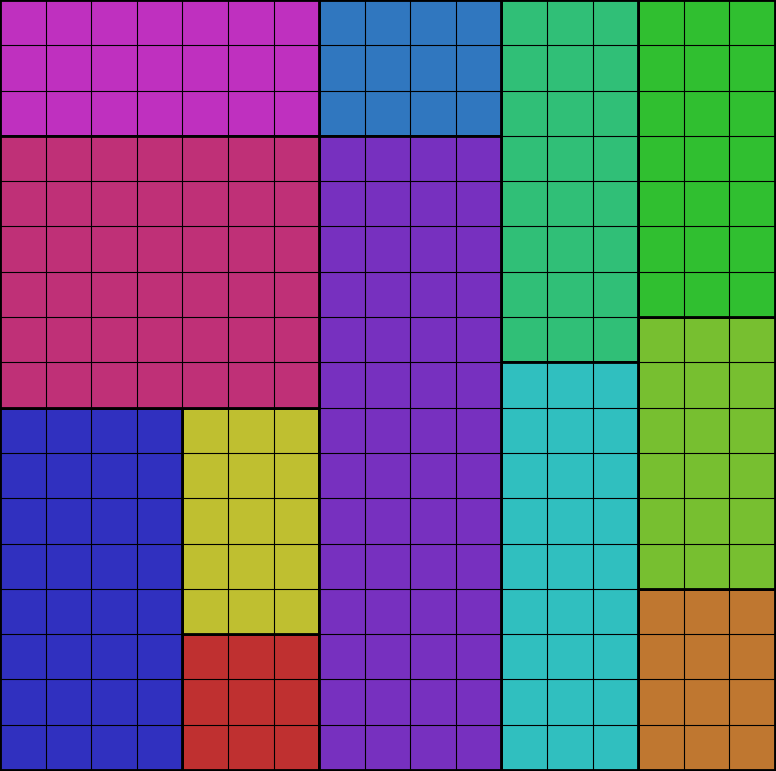
\includegraphics[width=0.618\textwidth]{Images/cover.png}}
\end{center}


\clearpage

\tableofcontents

\clearpage

\listoffigures

\clearpage


\section{Introduction}

\clearpage
\section{Modelling}\label{sec:modelling}


\subsection{Variables}

Each instance comes with 4 parameters describing the chip configuration:
\begin{itemize}
	\item \verb+chip_w+: the width of the chip;
	\item \verb+n+: the number of circuits to fit on the chip;
	\item \verb+inst_x+: a list containing the ordered widths of the circuits;
	\item \verb+inst_y+: a list containing the ordered heights of the circuits.
\end{itemize}
In addition, 3 auxiliary variables are created:
\begin{itemize}
	\item \verb+min_index+: the index of the smallest circuit (see Section \ref{sec:symmetry});
	\item \verb+min_h+: the minimum possible height of the chip (see Section \ref{sec:improvements});
	\item \verb+max_h+: the maximum possible height of the chip (see Sections \ref{sec:improvements}).
\end{itemize}
The results of the various solving procedures consists in 3 variables:
\begin{itemize}
	\item \verb+chip_h+: the height of the chip;
	\item \verb+bl_x+: a list containing the ordered horizontal positions of the bottom left corners of the circuits;
	\item \verb+bl_y+: a list containing the ordered vertical positions of the bottom left corners of the circuits.
\end{itemize}


\subsection{Constraints}

\subsubsection{Boundaries consistency}
Given the problem to fit all circuits into the chip, the first obvious constraint is that of not making the circuits fall out of the chip. This is quite easy: it is sufficient to impose that, for every circuit \verb|k|, both \verb|bl_x[k]| and \verb|bl_y[k]| to be non-negative, and the bottom right corner horizontal coordinate (\verb|bl_x[k] + inst_x[k]|) to be at most equal to the \verb|chip_w|.

\subsubsection{Non-overlapping}
The next step is to impose a non-overlapping constraint between each circuits' pair. In order to do that, the basic idea is to cycle through all the circuits and to check that the distance between every bottom left corner pair is at least equal to the dimension of the circuit in one direction.

\subsubsection{Symmetry breaking}\label{sec:symmetry}

In order to eliminate symmetrical solutions, a simple symmetry breaking constraint is introduced. As shown in Fig. \ref{fig:solutions}, each solution has four symmetrical configurations, where the circuits are located in symmetrical positions with respect to an horizontal and/or a vertical central symmetry ax.

\begin{figure}
    \centering
    \begin{subfigure}[t]{0.45\textwidth}
        \centering
        \fbox{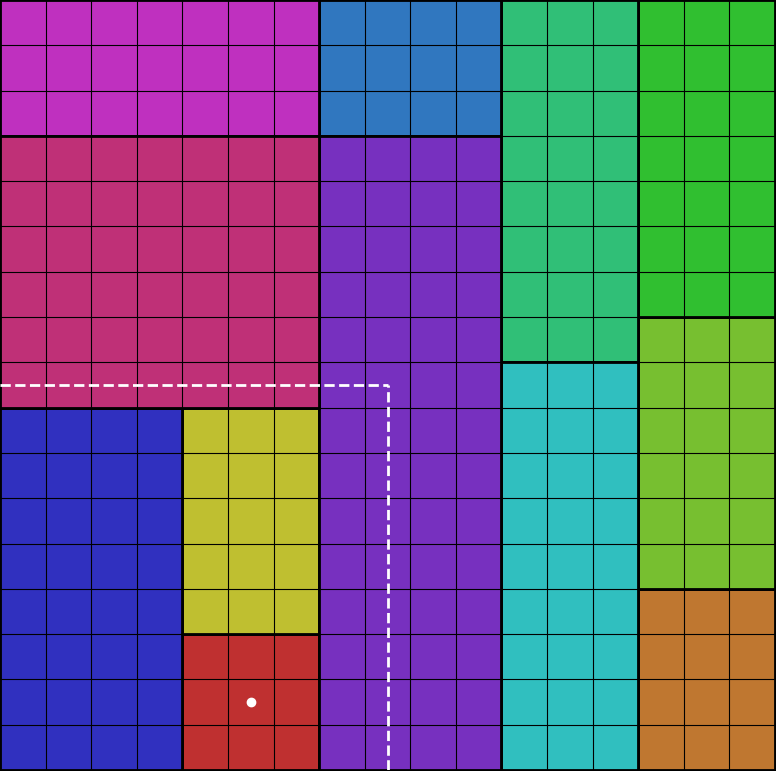
\includegraphics[width=\textwidth]{Images/symmetry-1.png}}
        \caption{Configuration 1.}
    \end{subfigure}
    \hfill
    \begin{subfigure}[t]{0.45\textwidth}  
        \centering 
        \fbox{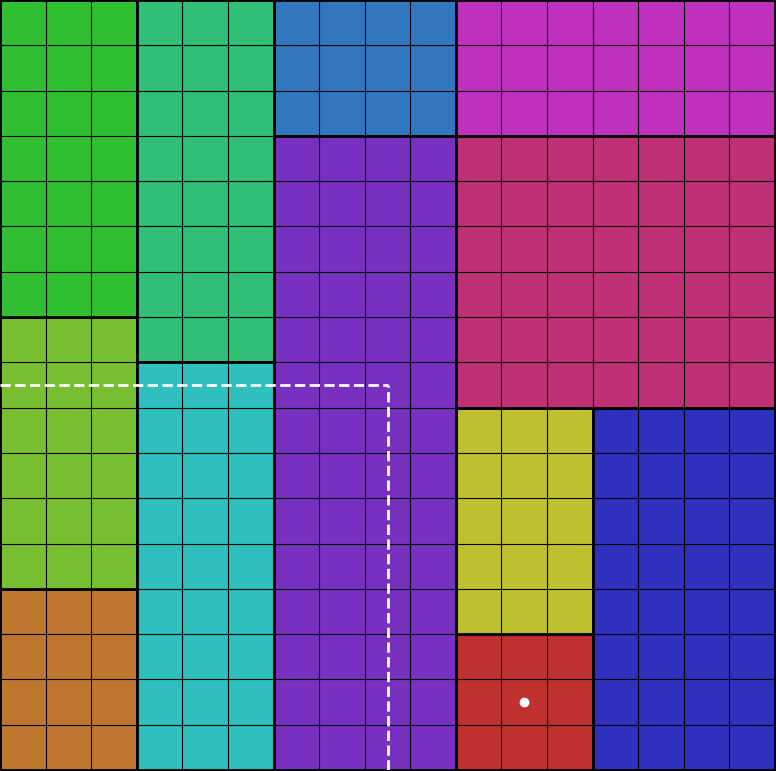
\includegraphics[width=\textwidth]{Images/symmetry-2.png}}
        \caption{Configuration 2.}
    \end{subfigure}
    \vskip\baselineskip
    \begin{subfigure}[t]{0.45\textwidth}   
        \centering 
        \fbox{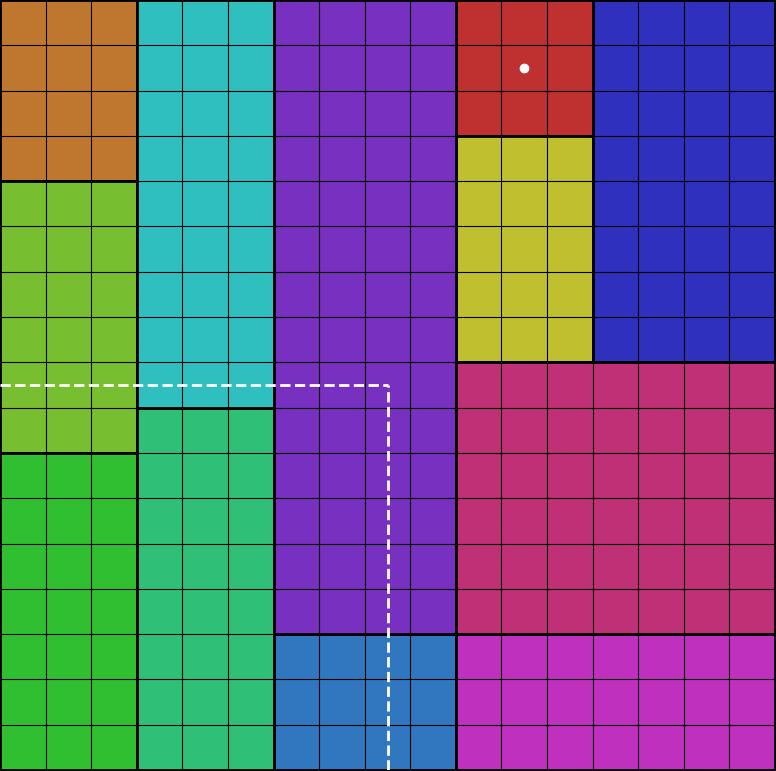
\includegraphics[width=\textwidth]{Images/symmetry-3.png}}
        \caption{Configuration 3.}
    \end{subfigure}
    \hfill
    \begin{subfigure}[t]{0.45\textwidth}   
        \centering 
        \fbox{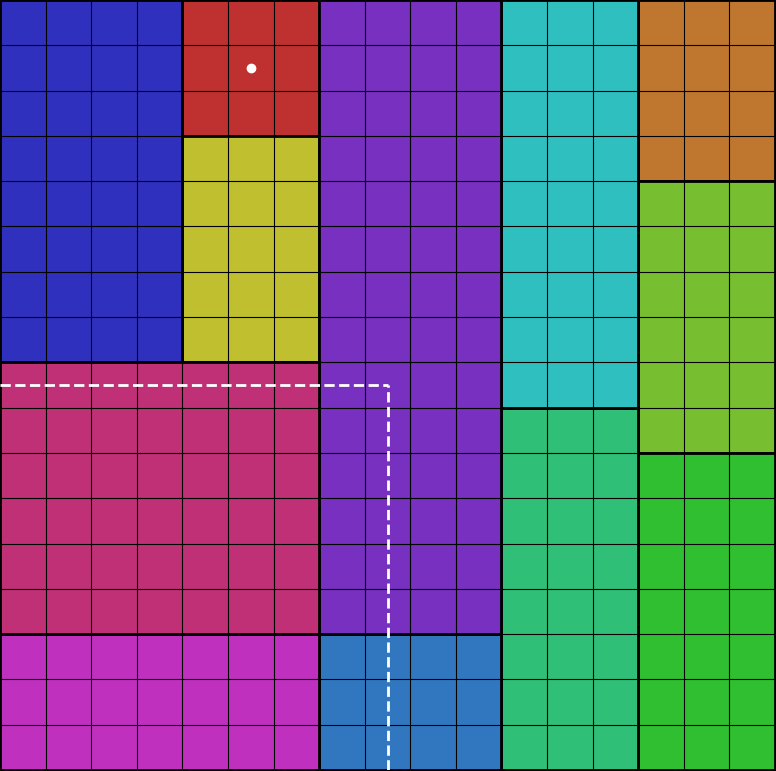
\includegraphics[width=\textwidth]{Images/symmetry-4.png}}
        \caption{Configuration 4.}
    \end{subfigure}
    \caption[Symmetrical configurations.]{Symmetrical configurations of Instance 10, with a white dot in the center of the smallest circuit and a dashed white line indicating the bottom left quadrant.}
    \label{fig:solutions}  
\end{figure}

In each of the configurations, the center of the smallest circuit (which has the index \verb|min_index|) is highlighted with a white dot and the bottom left quadrant is indicated by a dashed white line. It can be noted that the white dot lies in the highlighted quadrant in only one of the 4 symmetrical configurations, with the exception of very rare cases (i.e. when it lies exactly on the lines). Therefore, the chosen symmetry breaking constraint consists in forcing the white dot to lie in the bottom left quadrant.

\subsection{Rotation}


The next step is to implement circuit rotations. Since the circuits are rectangular and nothing is known \emph{a priori} about whether they would wedge perfectly without gaps keeping them in their base orientation, it may be possible that the minimal height of the chip is obtained by rotating some of the circuits. For example, the difference between the two solutions for Instance 10 is shown in Fig. \ref{fig:rotations}. Even if, at least for the given instance, rotating does not actually reduce the chip height, it can still be observed that some circuits get rotated by the solver.

\begin{figure}
    \centering
    \begin{subfigure}[t]{0.45\textwidth}
        \centering
        \fbox{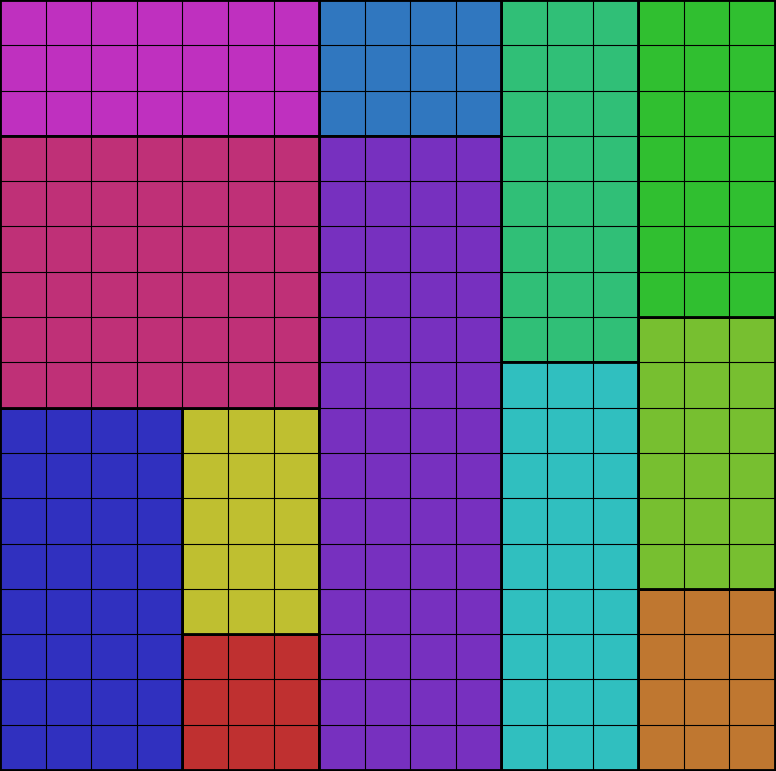
\includegraphics[width=\textwidth]{Images/cover.png}}
        \caption{Without rotations.}
    \end{subfigure}
    \hfill
    \begin{subfigure}[t]{0.45\textwidth}  
        \centering 
        \fbox{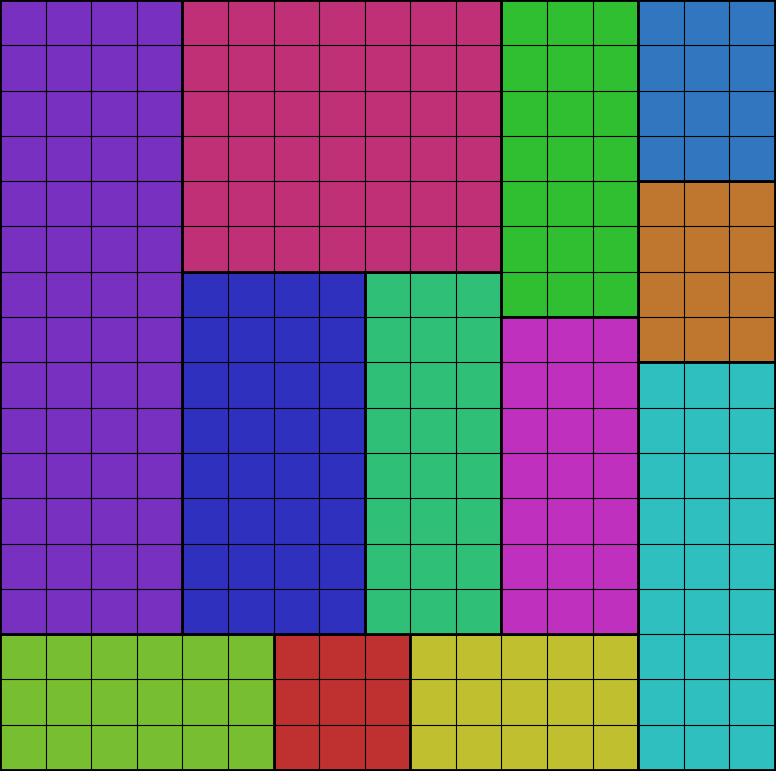
\includegraphics[width=\textwidth]{Images/rotated.png}}
        \caption{With rotations.}
    \end{subfigure}
    \caption[Solutions with and without rotations.]{Solutions of Instance 10 with and without enabled rotations.}
    \label{fig:rotations}  
\end{figure}

These rotations are handled differently in each implementation, but the basic idea is to offer both the normal and the rotated circuit to the solver and to impose an exclusive disjunction between the two orientations. In particular, it is useful to create 3 auxiliary variables:

\begin{itemize}
	\item \verb|rotated|: a boolean vector of flags signalling whether each circuit is rotated;
	\item \verb|new_inst_x|: a list containing the actual horizontal dimensions of the circuits;
	\item \verb|new_inst_y|: a list containing the actual vertical dimensions of the circuits;
\end{itemize}


This way, since boolean values are by nature exclusive, the dimensions of each circuit can be linked to the respective boolean value, effectively creating an exclusive disjunction between the two orientations.



\subsection{Improvements}\label{sec:improvements}

The main improvement of the model consists in adding boundaries to \verb|chip_h|. The minimum height is fairly easy to evaluate, since in the best case scenario (i.e. if the circuits leave no gaps) \verb|min_h = total_area / chip_w|, where \verb|total_area| is calculated by simply adding up all the products of the circuits' dimensions. Computing the maximum height, on the other hand, is more subtle. A naive approach consists in simply adding all heights together, considering the worst case as that where all circuits are stacked vertically. This is of course a reasonable upper boundary, but, as the number of circuits increases, \verb|max_h| greatly overestimates the actual height.

A more clever solution can be reached with minimal preprocessing reasoning as follows. If circuits are ordered by height and width, the following code can be run:
\begin{minted}[linenos]{python}
chip_cumulative = chip_w
k = 0
heights = []
while k < len(inst):
    if inst[k][0] <= chip_cumulative:
        chip_cumulative -= inst[k][0]
        heights.append(inst[k][1])
        del inst[k]
    else:
        k += 1
max_h += max(heights)
\end{minted}

The reasoning is the following. The circuits' widths are compared with the free horizontal space (\verb+chip_cumulative+) and, if each circuit fits, the free space is decreased. When no more circuits fit on the line, the maximum height is taken among the located circuits and it is added to the total \verb|max_h|. The process is then repeated for the next lines as long as there are circuits left. This way, a much more optimistic, but strictly valid, \verb|max_h| is computed, as shown in Fig. \ref{fig:max_h}.

\begin{figure}
    \centering
        \fbox{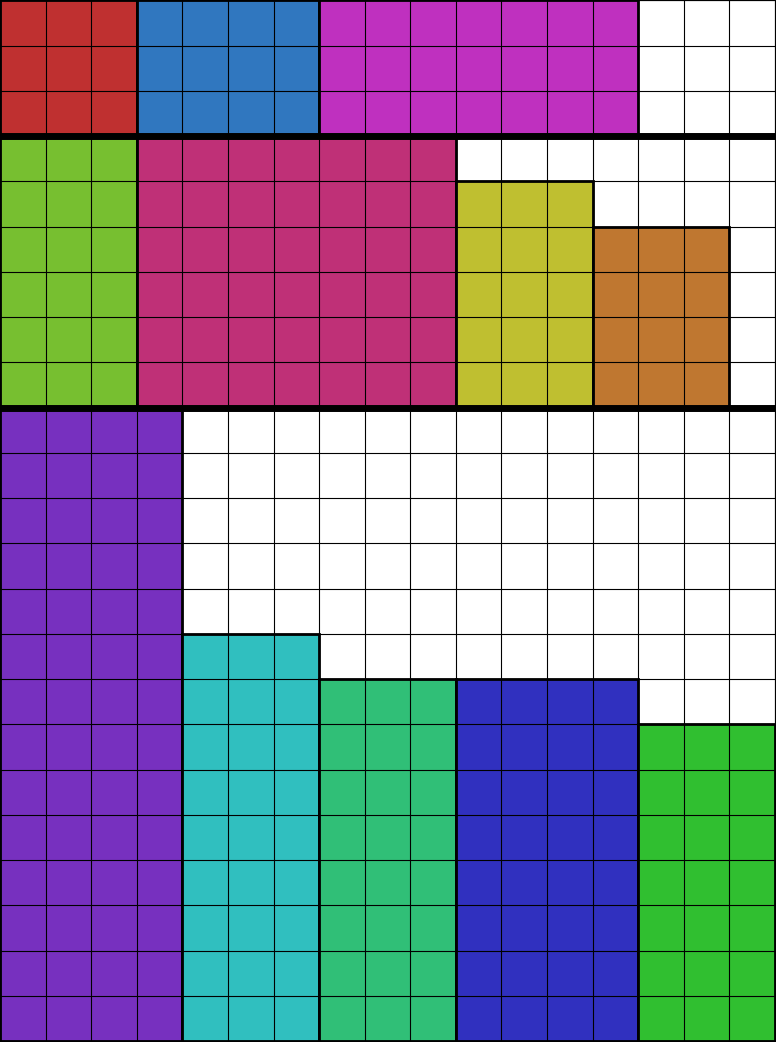
\includegraphics[width=\textwidth]{Images/max_h.png}}
        \caption[A graphical representation of the \texttt{max\symbol{95}h} algorithm.]{A graphical representation of the \texttt{max\symbol{95}h} algorithm for Instance 10.}
    \label{fig:max_h}  
\end{figure}


\clearpage

\section{Constraint Programming}
The first paradigm used to solve the combinatorial problem of \textsc{Vlsi} is Constraint Programming (CP), developed using MiniZinc as the modelling language. Two different models are used: \verb|cp_normal.mzn|, which solves the problem by using exactly the instances defined as input in the project, and \verb|cp_rotation.mzn| goes one step further, allowing also the rotation of the circuits themselves.

\subsection{Variables}
To start, \verb|cp_normal.mzn| it receives as input the variables \verb|chip_w|, \verb|n|, \verb|inst_x|, \verb|inst_y|, \verb|min_h|, \verb|max_h| and \verb|min_index|, already defined in Section \ref{sec:modelling}. Along with these variables, three additional variables are added to the output of the file:
\begin{itemize}
	\item \verb|bl_x|: array of size \verb|n| with domain \verb|0..(chip_w – min(inst_x))|, containing the horizontal coordinates of the bottom-left corners of the circuits;
	\item \verb|bl_y|: array of size \verb|n| with domain \verb|0..(max_h – min(inst_y))|, containing the vertical coordinates of the bottom-left corners of the circuits;
	\item \verb|chip_h|: variable with domain \verb|min_h..max_h| and which must be equal to the maximal circuit upper edge, this variable represents the effective height of the chip and is the objective function to minimize. 
\end{itemize}

\subsection{Constraints}
After having carried out a series of tests in which multiple constraints were developed and implemented together measuring the relative performances, the best model, consisting in four different constraints, was finally reached.


\subsubsection{Boundaries consistency}
This constraint ensures that no circuit is placed totally or partially outside the chip. Since MiniZinc does not provide any similar default predicate, the boundaries consistency constraint are implemented as follows:
\begin{minted}[linenos]{minizinc}
 constraint forall(i in RANGE) (
    (bl_x[i] + inst_x[i] <= chip_w) /\
    (bl_y[i] + inst_y[i] <= max_h));
 \end{minted}
 
 Using a \verb|forall| loop, it is verified that the sum of each circuit's bottom-left corner and its width or height is never greater than the width of the chip (\verb|chip_w|) or its maximum height (\verb|max_h|) respectively.


\subsubsection{Non-overlapping}
The non-overlapping constraint consists in imposing that the circuits within the chip do not overlap each other, ensuring that two different bottom-left corners do not have the same coordinates and that the circuits do not collide with each other. This constraint was implemented using as a global constraint the predicate \verb|diffn|, provided by MiniZinc, that performs exactly this check:
\begin{minted}[linenos]{minizinc}
constraint diffn(bl_x, bl_y, inst_x, inst_y);
 \end{minted}

This constraint and the boundaries consistency one are necessary and sufficient to solve the problem well.

\subsubsection{Cumulative}
An implied constraint was also added to the model to improve propagation. The \verb|cumulative| constraint is actually a scheduling constraint provided by MiniZinc and typically used to make sure that certain tasks do not overlap, but it adapts well to the \textsc{Vlsi} problem:
\begin{minted}[linenos]{minizinc}
constraint cumulative(bl_y, inst_y, inst_x, chip_w);
constraint cumulative(bl_x, inst_x, inst_y, max_h);
 \end{minted}
 
The MiniZinc reference manual explains how the cumulative constraint ``requires that a set of tasks given by start times s, durations d, and resource requirements r, never require more than a global resource bound b at any one time''. So, the first constraint requires that at any position along the horizontal axis, the required shared resource (i.e. the width of each circuit \verb|inst_x| in such position) of a circuit whose vertical coordinate is \verb|bl_y| and whose height is \verb|inst_y| never exceeds the width of the chip, \verb|chip_w|. The second constraint instead requires that at any position along the vertical axis, the required shared resource (i.e. the height of each circuit \verb|inst_y| in such position) of a circuit whose horizontal coordinate is \verb|bl_x| and whose width is \verb|inst_x| never exceeds the maximum height of the chip, \verb|max_h|.

\subsubsection{Symmetry breaking}

Finally, a symmetry breaking constraint was added. Its purpose is to avoid generating solutions that are symmetrical to each other, especially to prune branches of the solution tree that lead to non-acceptable states. As explained in Section \ref{sec:symmetry}, the goal of the symmetry breaking constraint is to force the center of the smallest circuit to be located in the lower left quadrant. To do so, \verb|min_index| is used to compute the center of the smallest circuit and to make sure that it lies in the lower-left quadrant, given by the half of the width and height of the chip:
\begin{minted}[linenos]{minizinc}
constraint symmetry_breaking_constraint(
    ((2 * bl_x[min_index] + inst_x[min_index]) <= chip_w) /\
    ((2 * bl_y[min_index] + inst_y[min_index]) <= chip_h));
 \end{minted}


\subsection{Rotation}
The problem requirements do not provide the possibility to rotate the circuits to perform a better placement inside the chip optimizing the height. To add this feature a new model called \verb|cp_rotation.mzn| is created, which is very similar to \verb|cp_normal.mzn| but with little few changes. A new array of booleans called \verb|rotated| is created, where the \verb|k|-th element is \verb|True| if the \verb|k|-th circuit must be rotated in the final result, \verb|False| otherwise. Two other arrays of integers called \verb|new_inst_x| and \verb|new_inst_y| are created, which contain the actual horizontal and vertical dimensions:
\begin{minted}[linenos]{minizinc}
array[RANGE] of var bool: rotated;
array[RANGE] of var int: new_inst_x;
array[RANGE] of var int: new_inst_y;
new_inst_x = [
    if rotated[k] then inst_y[k] else inst_x[k]
    endif | k in RANGE];
new_inst_y = [
    if rotated[k] then inst_x[k] else inst_y[k]
    endif | k in RANGE];
 \end{minted}
 
All previous constraints are then modified in such a way as to no longer use the default values of \verb|inst_x| and \verb|inst_y| but the actual dimensions \verb|new_inst_x| and \verb|new_inst_y|. Finally, since it is not possible to predict if a circuit will be rotated or not in the final solution, the domains of the variables \verb|bl_x| and \verb|bl_y| are updated, setting as upper limit the minimum value present indifferently in \verb|inst_x| or \verb|inst_y|, called \verb|min_size| and defined as:
\begin{minted}[linenos]{minizinc}
int: min_size = min(inst_x ++ inst_y);
 \end{minted}

 
\subsection{Search \& Restart}
MiniZinc provides to the users many different solvers and the possibility to use various type of search and restart algorithms. Among the natively available solvers, only two are based on CP: Gecode and Chuffed. The latter was used, because as explained by the reference manual of MiniZinc it is based on lazy clause generation and adapts techniques from SAT solving as activity-based search heuristic. In order to take full advantage of Chuffed’s performance, the Free search option is used: this allows the solver to switch between the search exploiting annotations and the activity-based one. Then, in order to optimize the solver at its best, an optimization level O5 is used: this performs root-node-propagation with Gecode and probe values of all variables at the root node. With this kind of settings, different types of variable choice annotations were tested. Search annotations in MiniZinc specify how to search in order to find a solution to the problem. The annotation is attached to the solve item, after the keyword \verb|solve|. Six different types of annotations were tried:
\begin{itemize}
	\item \verb|(input_order, indomain_min)|: chooses the variable in order from array, assigns to each variable its smallest domain value;
	\item \verb|(first_fail, indomain_min)|: chooses the variable with the smallest domain size, assigns to each variable its smallest domain value;
	\item \verb|(dom_w_deg, indomain_min)|: chooses the variable with the smallest value of domain size divided by weighted degree, which is the number of times it has been in a constraint that caused failure earlier in the search, assigns to each variable its smallest domain value;
	\item \verb|(input_order, indomain_random)|: chooses variables in order from array, assigns to each variable a random value from its domain;
	\item \verb|(first_fail, indomain_random)|: chooses the variable with the smallest domain size, assigns to each variable a random value from its domain;
	\item \verb|(dom_w_deg, indomain_random)|: chooses the variable with the smallest value of domain size divided by weighted degree, which is the number of times it has been in a constraint that caused failure earlier in the search, assigns to each variable a random value from its domain.
\end{itemize}

Any kind of depth-first search for solving optimization problems suffers from the problem that wrong decisions made at the top of the search tree can take an exponential amount of search to undo. One common way to avoid this problem is to restart the search from the top thus having a chance to make different decisions. MiniZinc includes annotations to control restart behaviour. These annotations, like other search annotations, are attached to the solve item of the model. The different restart annotations control how frequently a restart occurs. Restarts occur when a limit in nodes is reached, where search returns to the top of the search tree and begins again. Four different types of restart annotations were tried:
\begin{itemize}
	\item \verb|restart_constant(<scale>)|: where \verb|<scale>| is an integer defining after how many nodes to restart;
	\item \verb|restart_linear(<scale>)|: where \verb|<scale>| is an integer defining the initial number of nodes before the first restart, the second restart gets twice as many nodes, the third gets three times, etc.;
	\item \verb|restart_geometric(<base>,<scale>)|: where \verb|<base>| is a float and \verb|<scale>| is an integer, the \verb|k|-th restart has a node limit of $\texttt{<scale>} \cdot \texttt{<base>}^\texttt{k}$;
	\item \verb|restart_luby(<scale>)|: where \verb|<scale>| is an integer, the \verb|k|-th restart gets \verb|<scale> * L[k]| where \verb|L[k]| is the \verb|k|-th number in the Luby sequence, which looks like 1 1 2 1 1 2 4 1 1 2 1 1 2 4 8 …, i.e. it repeats two copies of the sequence ending in $2^\texttt{k}$ before adding the number $2^{\texttt{k}+1}$.
\end{itemize}
Combining different types of search and restart strategies it was found that the best possible combination is formed by \verb|first_fail| as variable choice, \verb|indomain_min| as variable constraint and \verb|restart_luby(250)| as restart type.

\subsection{Results}
As shown in Fig. \ref{fig:cp}, the normal model without rotations solves all input instances except 30, 37 and 40 with a maximum time of around minutes. The addition of the symmetry breaking constraint allowed to solve some instances that previously could not be solved, also speeding up the resolution time in general and reducing the number of nodes in the tree, proving that it works properly. By adding the ability to rotate the circuits in the solutions, slightly worse times are obtained instead. This behavior was predictable since the solver must in this case perform many more combinations. Also, since each instance already allowed for the minimum chip height without the rotation, adding the rotation did not lead to better results either. The model with rotation therefore solves the same instances of \verb|cp_normal.mzn|, except for 22, 25, 32, 38, and 39, always with a maximum time of two minutes.

\begin{figure}
    \centering
        \fbox{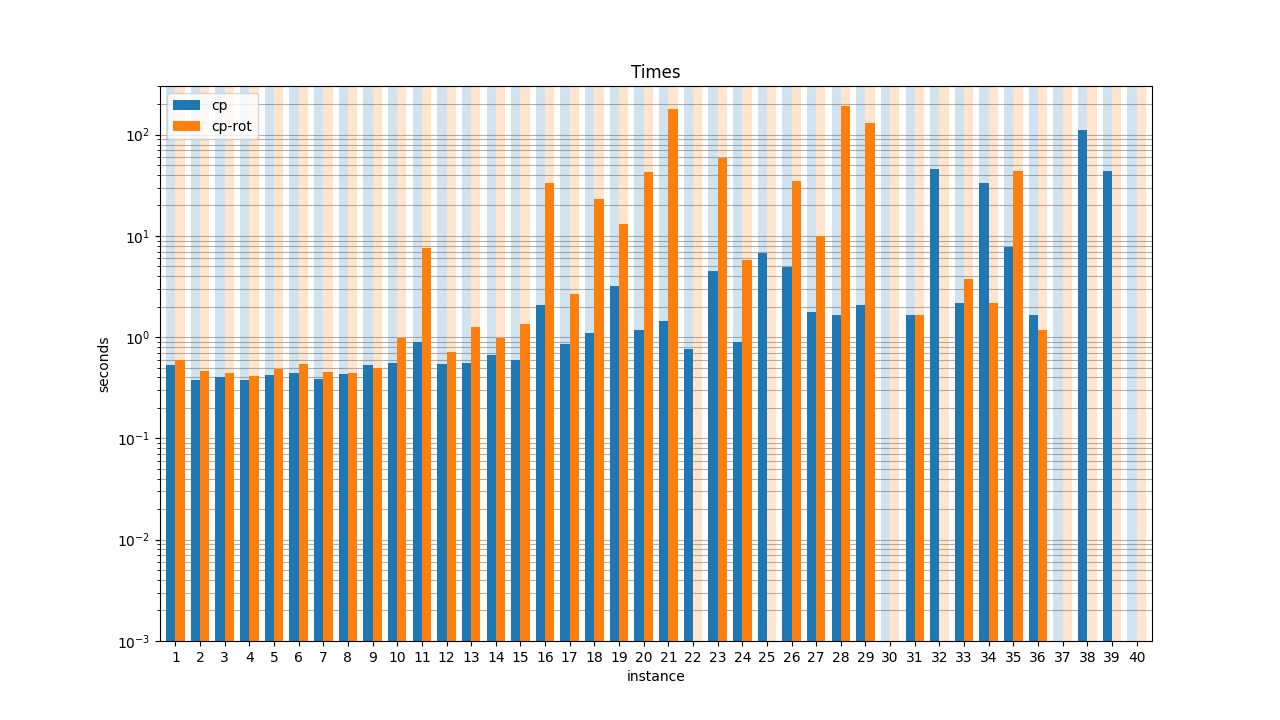
\includegraphics[width=\textwidth]{Images/times-cp.png}}
        \caption{Constrain Programming times}
    \label{fig:cp}  
\end{figure}



\clearpage

\section{Propositional Satisfiability}
The second paradigm used to solve the combinatorial problem of \textsc{Vlsi} is Propositional SATisfiability (SAT), developed using the z3 Python package.



\subsection{Variables}
To start, the solver receives as input the variables \verb|chip_w|, \verb|n|, \verb|inst_x|, \verb|inst_y|, \verb|min_h|, \verb|max_h| and \verb|min_index|, already defined in Section \ref{sec:modelling}. Along with these variables, 3 auxiliary variables are defined:
\begin{itemize}
	\item \verb|chip|: a $\texttt{chip\symbol{95}w} \times \texttt{max\symbol{95}h} \times \texttt{n}$ matrix of booleans where any element \verb|chip[i][j][k]| is \verb|True| if circuit \verb|k| is present at coordinates \verb|(i,j)|, \verb|False| otherwise;
	\item \verb|corners|: a $\texttt{chip\symbol{95}w} \times \texttt{max\symbol{95}h} \times \texttt{n}$ matrix of booleans where any element \verb|corners[i][j][k]| is \verb|True| if the corners of circuit \verb|k| has coordinates \verb|(i,j)|, \verb|False| otherwise;
	\item \verb|chip_h|: integer variable which represents the effective height of the chip and is the objective function to minimize. 
\end{itemize}


\subsection{Constraints}
After having carried out a series of tests in which multiple constraints were developed and implemented together measuring the relative performances, the best model was finally reached.

\subsubsection{Structural}
Contrary to the other paradigms, SAT requires some structural constraints. This is necessary because, dealing with boolean matrices, the concepts of height and width occupied by each chip is not so simply manageable. The way it is done is by cycling first among all the circuits and creating a list of booleans \verb|temp_corners|. Then, for every coordinate, another list of booleans \verb|temp| is created. Next, all coordinates are cycled through again inside the higher-level cycle, in order to effectively have all possible coordinates' pairs. At this point, it is checked whether the new coordinates \verb|ii| and \verb|jj| would be part of the circuit if its coordinates were \verb|i| and \verb|j|: if this is the case, an implication constraint is added, signifying that, in case \verb|(i,j)| become the location of the corner of chip \verb|k|, then \verb|chip[ii][jj][k]| must also be true. In addition, for every circuit, it is imposed that only one position can be occupied by the corner, as indicated by the last two lines of code:
\begin{minted}[linenos]{python}
for k in range(n):
    temp_corners = []
    for i in range(chip_w):
        for j in range(max_h):
            temp = []
            for ii in range(chip_w):
                for jj in range(max_h):
                    if (ii in range(i, i + inst_x[k])
                        and jj in range(j, j + inst_y[k])):
                        temp.append(chip[ii][jj][k])
                    else:
                        temp.append(Not(chip[ii][jj][k]))
            opt.add(Implies(corners[i][j][k], And(temp)))
            temp_corners.append(corners[i][j][k])
    opt.add(at_least_one(temp_corners))
    opt.add(at_most_one(temp_corners))
\end{minted}


\subsubsection{Boundaries consistency}
The boundaries consistency constraint is created by cycling through all the coordinates and all the circuits and imposing that, if corner \verb|k| is at coordinates \verb|(i,j)|, then both coordinates, summed with the circuit's dimensions, must be at most equal to the chip dimensions:
\begin{minted}[linenos]{python}
for i in range(chip_w):
    for j in range(max_h):
        for k in range(n):
            opt.add(Implies(
                corners[i][j][k],
                And(i <= chip_w - inst_x[k],
                    j <= chip_h - inst_y[k])))
\end{minted}

\subsubsection{Non-overlapping}
Non-overlapping is achieved in a very straightforward way for both \verb|chip| and \verb|corners|. First, both dimensions are cycled and 2 lists of booleans are created. Then, it is imposed that only one circuit (or corner) can be present at each spatial position:
\begin{minted}[linenos]{python}
for i in range(chip_w):
    for j in range(max_h):
        temp_chip = []
        temp_corners = []
        for k in range(n):
            temp_chip.append(chip[i][j][k])
            temp_corners.append(corners[i][j][k])
        opt.add(at_most_one(temp_chip))
        opt.add(at_most_one(temp_corners))
\end{minted}



\subsubsection{Symmetry breaking}
Symmetry breaking is achieved in the same way as when using the other approaches: it is imposed that the center of the smallest circuit lies in the bottom left quadrant of the chip. In order to do so, the code first creates an empty list \verb|symmetry_breaking| and then cycles all the spatial positions. At this point, it is imposed, using conjunctions, that the center of the smallest circuit lies in the bottom left quadrant of the chip:
\begin{minted}[linenos]{python}
symmetry_breaking = []
for i in range(chip_w):
    for j in range(max_h):
        symmetry_breaking.append(And(
            corners[i][j][min_index],
            And(
                2 * i + inst_x[min_index] <= chip_w,
                2 * j + inst_y[min_index] <= chip_h)))
opt.add(Or(symmetry_breaking))
\end{minted}

Even if, at first glance, it may seem that using a conjunction is wrong, since of course the corner is not at all positions at the same time, the elements of \verb|symmetry_breaking| are actually added as a disjunctive constraint, therefore effectively forcing the center \emph{at least} once in the quadrant. But of course, the center can occupy only one position at a time, thanks to the non-overlapping constraint.

\subsection{Rotation}
To deal with rotation, a new list of booleans called \verb|rotated| is created, where the \verb|k|-th element is \verb|True| if the \verb|k|-th circuit must be rotated in the final result, \verb|False| otherwise. Two other arrays called \verb|new_inst_x| and \verb|new_inst_y| are created as well, which contain the actual horizontal and vertical dimensions:
\begin{minted}[linenos]{python}
rotated = BoolVector("rotated", n)
new_inst_x = [If(rotated[k], inst_y[k], inst_x[k])
    for k in range(n)]
new_inst_y = [If(rotated[k], inst_x[k], inst_y[k])
    for k in range(n)]
 \end{minted}
 
All previous constraints are then modified in such a way as to no longer use the default values of \verb|inst_x| and \verb|inst_y| but the actual dimensions \verb|new_inst_x| and \verb|new_inst_y|.

\subsection{Results}
As shown in Fig. \ref{fig:sat}, SAT performs pretty badly compared to the other methods: the normal model without rotations only solves instances from 1 to 9, with the rotation model solving only the first 7.

\begin{figure}
    \centering
        \fbox{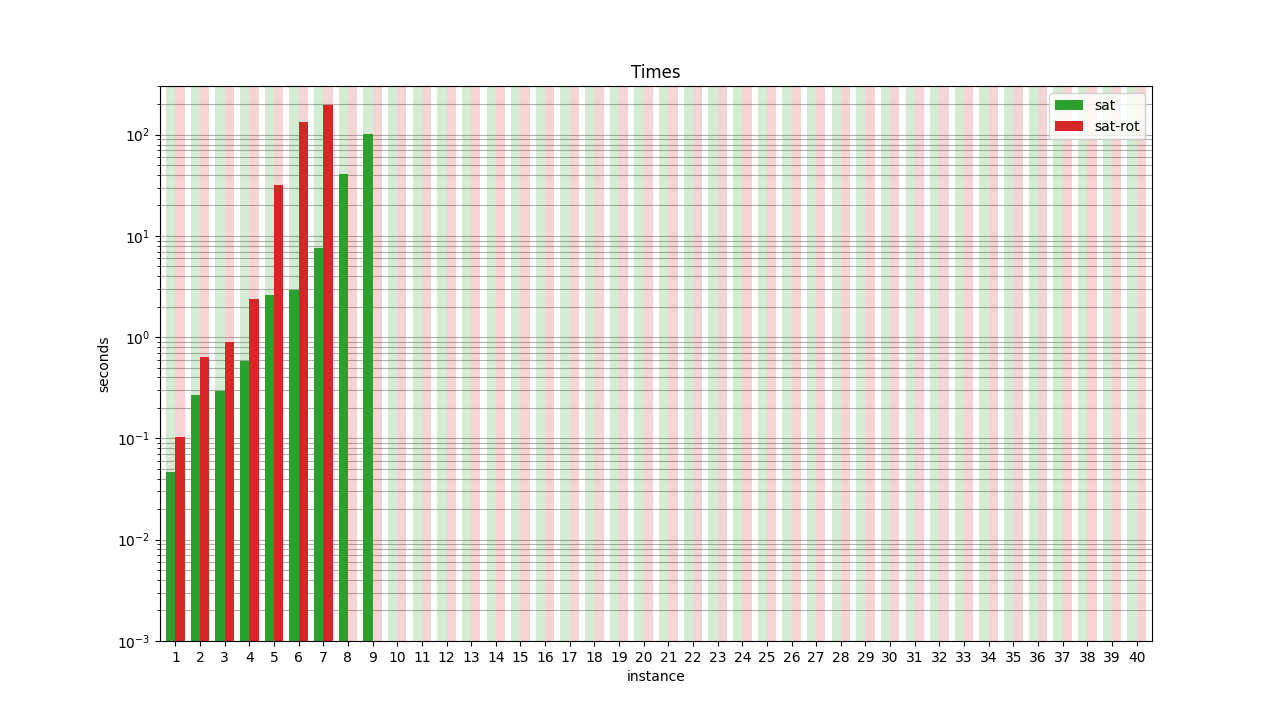
\includegraphics[width=\textwidth]{Images/times-sat.png}}
        \caption{Propositional Satisfiability times}
    \label{fig:sat}  
\end{figure}




\clearpage

\section{Satisfiability Modulo Theories}

\subsection{Variables}
\subsection{Constraints}
\subsection{Rotation}
\subsection{Improvements}

\clearpage

\section{Results}

\subsection{Normal}
\subsection{Rotated}

\end{document}



















